\documentclass{beamer} % "Beamer" is a word used in Germany to mean video projector. 

\usetheme{Berlin} % Search online for beamer themes to find your favorite or use the Berkeley theme as in this file.
\usepackage[slovene]{babel}
\usepackage[cp1250]{inputenc}
\usepackage{color} % It may be necessary to set PCTeX or whatever program you are using to output a .pdf instead of a .dvi file in order to see color on your screen.
\usepackage{graphicx} % This package is needed if you wish to include external image files.
\usepackage{wrapfig}

\usepackage{amsmath,amssymb,amsfonts}
\usepackage{url}
\usepackage{authblk}
% ukazi za matematicna okolja
\theoremstyle{definition} % tekst napisan pokoncno
\newtheorem{definicija}{Definicija}[section]
\newtheorem{primer}[definicija]{Primer}
\newtheorem{opomba}[definicija]{Opomba}

\renewcommand\endprimer{\hfill$\diamondsuit$}


\theoremstyle{plain} % tekst napisan posevno
\newtheorem{lema}[definicija]{Lema}
\newtheorem{izrek}[definicija]{Izrek}
\newtheorem{trditev}[definicija]{Trditev}
\newtheorem{posledica}[definicija]{Posledica}


% za stevilske mnozice uporabi naslednje simbole
\newcommand{\R}{\mathbb R}
\newcommand{\N}{\mathbb N}
\newcommand{\Z}{\mathbb Z}
\newcommand{\C}{\mathbb C}
\newcommand{\Q}{\mathbb Q}


% ukaz za slovarsko geslo
\newlength{\odstavek}
\setlength{\odstavek}{\parindent}
\newcommand{\geslo}[2]{\noindent\textbf{#1}\hspace*{3mm}\hangindent=\parindent\hangafter=1 #2}



%\theoremstyle{definition} % See Lesson Three of the LaTeX Manual for more on this kind of "proclamation."
%\newtheorem*{dfn}{A Reasonable Definition}               
\begin{document}
\title{Skriti markovski modeli v finan�nih �asovnih vrstah}
%\newcommand{\imeavtorja}{Martin Pra�ek} % ime avtorja
%\newcommand{\imementorja}{izr. prof. dr. Damjan Škulj}
\institute{Fakulteta za matematiko in fiziko, Univerza v Ljubljani}
%\date{January 6, 2012} 
% Remove the % from the previous line and change the date if you want a particular date to be displayed; otherwise, today's date is displayed by default.

%\AtBeginSection[]  % The commands within the following {} will be executed at the start of each section.
%{%
%\begin{frame} % Within each "frame" there will be one or more "slides."  
%\frametitle{} % This is the title of the outline.
%\tableofcontents[currentsection]  % This will display the table of contents and highlight the current section.
%\end{frame}
%} % Do not include the preceding set of commands if you prefer not to have a recurring outline displayed during your presentation.
\begin{frame} 
\includegraphics[scale=0.4]{slike/slucajni}
\end{frame}


\begin{frame} 
\begin{titlepage}
	\begin{center}
		\vspace*{1cm}
		Martin Pra�ek \\
		Mentor: izr. prof. dr. Damjan �kulj
		
		\vspace{3cm}
		
\includegraphics[scale=1]{slike/logo}
		
		
		\vfill
		
		\large Ljubljana, december 2018
		
	\end{center}
\end{titlepage}
\end{frame}

%\section{Markovski model} % Since this is the start of a new section, our recurring outline will appear here.


\begin{frame} 
\frametitle{Markovska lastnost}
\begin{definicija}{Markovska lastnost}\label{markov}
	Naj bo $(\Omega,\mathcal{F},\mathbb{P},\mathcal{F}_s)$ verjetnostni prostor s filtracijo za neko urejeno mno�ico $I$. Naj bo $(S,\mathcal{S})$ merljiv prostor. $(S,\mathcal{S})$ merljiv slu�ajni proces $X=\{X_t:\Omega \to S\}_{t\in I}$, ki je prilagojen na filtracijo, ima markovo lastnost, �e za vsak $A \in \mathcal{S}$ in vsak $s,t\in I$, kjer velja $s,t$ velja $$\mathbb{P}(X_t \in A \mid \mathcal{F}_s) = \mathbb{P}(X_t \in A\mid X_s)$$
\end{definicija}
\end{frame}

\begin{frame} 
\begin{opomba}
	$\mathbb{P}(X_n=x_n\mid X_{n-1}=x_{n-1}, \dots, X_0=x_0)=$ $$\mathbb{P}(X_n=x_n\mid X_{n-1}=x_{n-1})$$
\end{opomba}
\end{frame}

\begin{frame} 
\begin{table}
	\begin{tabular}{lllll}
		\cline{1-3}
		\multicolumn{1}{|c|}{}            & \multicolumn{1}{c|}{V celoti opazovan}         & \multicolumn{1}{c|}{Le delno opazovan} \\ \cline{1-3}
		\multicolumn{1}{|c|}{Avtonomen}   & \multicolumn{1}{c|}{Markovska veriga} & \multicolumn{1}{c|}{Skriti markovski model}    \\ \cline{1-3}
		\multicolumn{1}{|c|}{Kontorliran} & \multicolumn{1}{c|}{Markovski proces odlo�anja} & \multicolumn{1}{c|}{Delno opazovan proces}   \\ \cline{1-3}
		&                                &                             &           &         
	\end{tabular}
\end{table}
\end{frame}

\begin{frame} 

\includegraphics[scale=1]{slike/zaba}
\end{frame}

\begin{frame} 
\frametitle{Skriti markovski model}
\begin{itemize}
	\item Bayesianska mre�a
	\item Viterbi
\end{itemize}
\includegraphics[scale=0.5]{slike/circuits}
\end{frame}

\begin{frame}
\frametitle{Druge vrste skritih markovskih modelov}
\begin{enumerate}
	\item Zvezni primeri
	\item Odvisno od ve� spremenljivk
\end{enumerate}
\end{frame}

\begin{frame} 
\frametitle{Zgodovina}
\includegraphics[scale=0.8]{slike/onjegin2}
\end{frame}


\begin{frame}
\frametitle{Zgodovina}
\begin{wrapfigure}{r}{0.5\textwidth}
	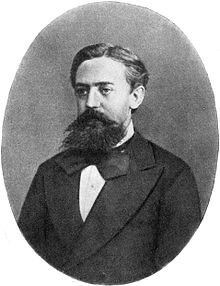
\includegraphics[scale=0.5]{slike/AAMarkov}
\end{wrapfigure}
\begin{itemize}
	\item Matemati�na teorija komunikacije
	\item EM-algoritem
	\item Stratonovi�
	\item Viterbi
	\item Baum-Welch
	\item James Hamilton
\end{itemize}

\end{frame}

\begin{frame}
\frametitle{Zahteve}
\begin{itemize}
	\item Markovska lastnost
	\item Enakomerno porazdeljeni �asi signalov $O_{t}$, ki jih poda resni�ni svet
	\item Sistem ima $N$ stanj, vsako dolo�a slu�ajna spremenjivka $S$
\end{itemize}
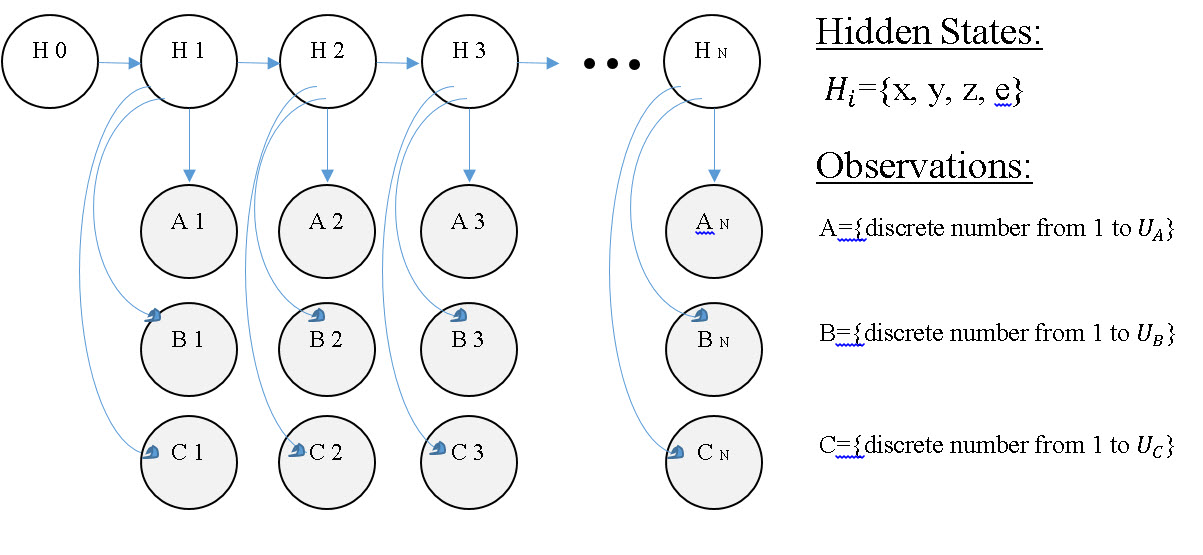
\includegraphics[scale=0.25]{slike/hmm}
\end{frame}

\begin{frame}
\begin{itemize}
\item Slu�ajnih spremenljivk skritih skoraj v nobenem �asu ne poznamo, poznamo pa slu�ajni proces $Q$, ki predstavlja signale
\item Porazdelitveni zakon vsakega stanja $i$ ozna�imo z $b_{i}(x)$
\item Vektor za�etnih stanj je $\pi$
\item Prehodna matrika $A$, ki je neodvisna od �asa
\end{itemize}
\end{frame}

\begin{frame}
\frametitle{Porazdelitveni zakon}
\begin{itemize}
\item Gaussova me�anica
\item  $b_{i} = \sum_{j = 1}^{M}{c_{ij}} N(x;\mu_{j}, \sigma_{j}^2)$
\item �tevilo porazdelitev $M$
\item Matrika $\Gamma$, $\mu_{ij}$ predstavlja pri�akovano vrednost porazdelitve $j$ v stanju $i$
\item Matrika $\Sigma$, kjer $\sigma_{ij}$ predstavlja varianco porazdelitve $j$ v stanju $i$
\item Matrika $C$, koeficienti $c_{ij}$ iz Gaussove me�anice
\end{itemize}
\end{frame}

\begin{frame} 
\frametitle{Generiranje poti v skritem markovskem modelu}
\begin{itemize}
	\item $O = (O_1,\ldots, O_T)$
	\item $\lambda$ $=$ $(\Pi,A,C,\Gamma,\Sigma)$
	\item $P(O|\lambda)$
	\item Za�etno stanje
\end{itemize}
\end{frame}

\begin{frame} 
\frametitle{Uporaba}
\begin{itemize}
	\item Biologija
	\item Procesiranje govora
	\item Prepozavanje akcij
	\item Kriptoanaliza
\end{itemize}
\end{frame}

\begin{frame} 
\frametitle{�asovne vrste}
\begin{definicija}{�asovna vrsta} mno�ica opazovanj $x_t$, vsako opazovano ob �asih $t$ znotraj nekega �asovnega intervala.
\end{definicija}

\begin{definicija}{Model �asovne vrste} za opazovane podatke ${x_t}$ je slu�ajni proces $X_t$, kjer velja, da so $x_t$ realizacije tega slu�ajnega procesa v �asih $t$.\\
\end{definicija}
\end{frame}

\begin{frame} 
\begin{itemize}
	\item Analiti�na ali prediktivna
	\item Odvisne od �asa
	\item Odvisnost
\end{itemize}
\end{frame}

\begin{frame} 
\begin{itemize}
	\item Diskreten �as
	\item Zvezen �as
	\item Diskretne vrednosti
\end{itemize}
\end{frame}

\begin{frame} 
\begin{definicija}{Finan�na �asovna vrsta} je �asovna vrsta, kjer so opazovanja $x_t$ vrednosti finan�nega instrumenta v �asu $t$.
\end{definicija}
\begin{itemize}
	\item Normalna porazdelitev donosov 
\end{itemize}
\end{frame}

\begin{frame} 
\frametitle{Uporaba skritih markovskih modelov v finan�nih �asovnih vrstah}
\begin{itemize}
	\item Zaporedje cen $O$
	\item Finan�na optimizacija
\end{itemize}
\end{frame}

\begin{frame} 
\frametitle{Problem izbire portfelja}
\begin{itemize}
	\item Kapital $M$
	\item $N$ vrednostnih papirjev
	\item Vsak papir ima donos $R_j$
	\item $R_x = \sum_{j=1}^{N}{x_jR_j}$
	\item $d$ zahtevan donos
	\item $\alpha$ stopnja zavrnitve
\end{itemize}
\end{frame}


\begin{frame} 
\begin{gather*}
\min \quad CVaR_\alpha(R_x) \\
\begin{aligned}
\textup{p.p.}\quad E(R_x) \geq d \\
\end{aligned}
\end{gather*}

\end{frame}
\frametitle{Prakti�ni primer}
\begin{frame}
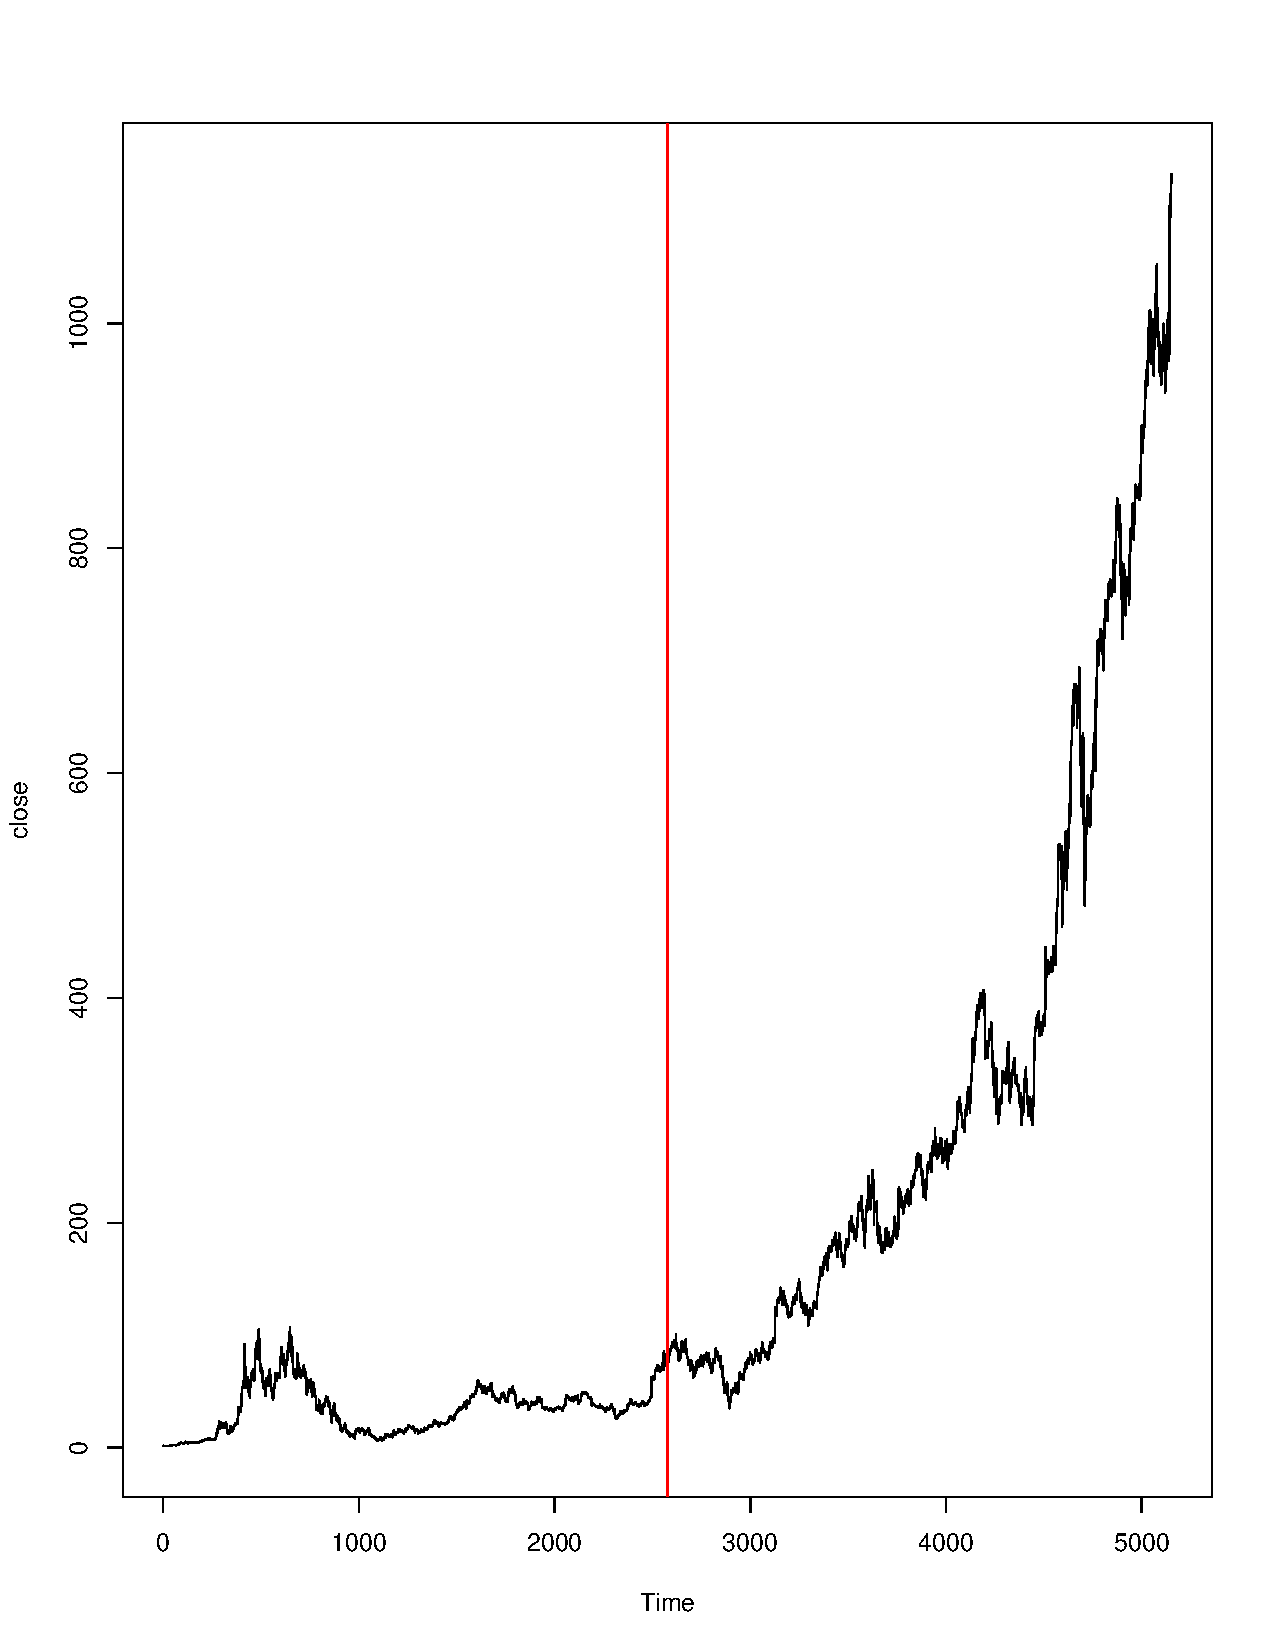
\includegraphics[scale=0.2]{slike/celota}
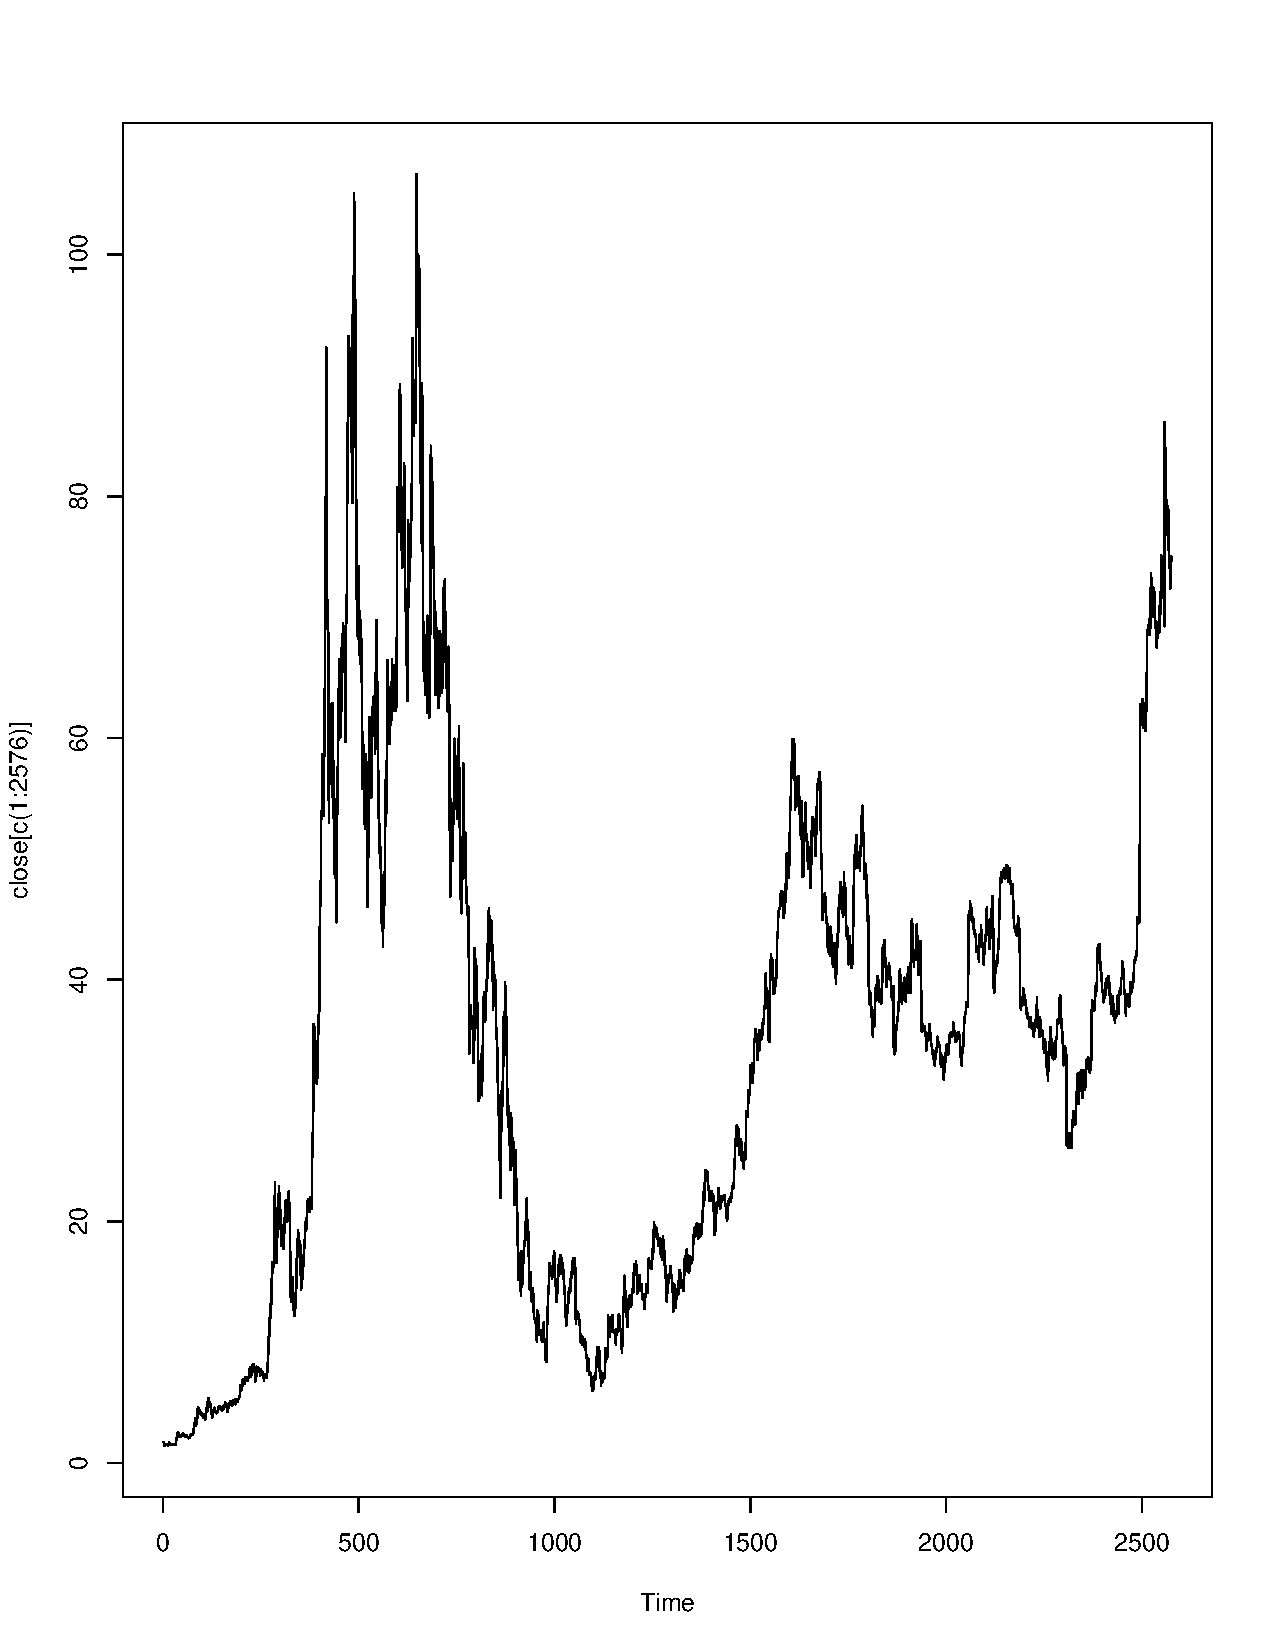
\includegraphics[scale=0.2]{slike/polovica}
\end{frame}

\begin{frame} 
\begin{itemize}
	\item Amazon
	\item Google
	\item Tesla
	\item TripAdvisor
	\item Starbucks
	\item Novartis
	\item Microsoft
	\item General Motors
	\item Wells Fargo
	\item Chevron
\end{itemize}
\end{frame}

\begin{frame}
\frametitle{Viri}
	\begin{thebibliography}{9}
		\bibitem{prvivir}
		D.~Roman, G.~Mitra in N.~Spagnolo, \emph{Hidden Markov models for financial optimization problems}, IMA Journal of Management Mathematics \textbf{21} (2010) 111--129.
		
		\bibitem{macdonald}
		I.L.~MacDonald in W.~Zucchini, \emph{Hidden Markov and Other Models for Discrete- valued Time Series}, Chapman \& Hall/CRC Monographs on Statistics \& Applied Probability  \textbf{70}, Chapman \& Hall, London, 1997.
		
		\bibitem{mamon}
		R.S.~Mamon in R.J.~Elliott \emph{Hidden Markov Models in Finance}, International Series in Operations Research \& Management Science  \textbf{104}, Springer, New York, 2007.
		
		\bibitem{davis}
		P.J.~Brockwell, R.A.~Davis \emph{Introduction to Time Series and Forecasting},2nd edition, Springer, 2002.
		
\end{thebibliography}		 
\end{frame}

\begin{frame} 
\frametitle{Markovski model}
\end{frame}


\end{document}

